%%%%%%%%%%%%%%%%%%%%%%%%%%%%%%%%%%%%%%%%%%%%%%%%%%%%%%%%%%%%%%%%%%%%%%%%%%%
%%
%% Copyright (c) 2014 Adobe Systems Incorporated. All rights reserved.
%%
%% Licensed under the Apache License, Version 2.0 (the "License");
%% you may not use this file except in compliance with the License.
%% You may obtain a copy of the License at
%%
%% http://www.apache.org/licenses/LICENSE-2.0
%%
%% Unless required by applicable law or agreed to in writing, software
%% distributed under the License is distributed on an "AS IS" BASIS,
%% WITHOUT WARRANTIES OR CONDITIONS OF ANY KIND, either express or implied.
%% See the License for the specific language governing permissions and
%% limitations under the License.
%%
%%%%%%%%%%%%%%%%%%%%%%%%%%%%%%%%%%%%%%%%%%%%%%%%%%%%%%%%%%%%%%%%%%%%%%%%%%%
\documentclass{beamer}
% Theme Matrix: http://www.hartwork.org/beamer-theme-matrix/
\mode<presentation> { \usetheme{Malmoe}\usecolortheme{dove} }
\setbeamertemplate{itemize items}[default]
\usepackage[T1]{fontenc}
\usepackage{parskip,graphics,tikz,multimedia,hyperref,ulem,multicol}
\usetikzlibrary{arrows,positioning,shapes,decorations.pathmorphing,
  decorations.markings}
\setlength{\itemsep}{0pt}\setlength{\parskip}{0pt}\setlength{\parsep}{0pt}
\graphicspath{{./images/}}

\usepackage{listings,textcomp,color}
\lstset{language=Python,upquote=true,
  basicstyle=\ttfamily\tiny,numbers=left,
  numberstyle=\tiny,stepnumber=1,numbersep=5pt,
  backgroundcolor=\color{white},frame=single,tabsize=2,
  showspaces=false,showstringspaces=false,showtabs=false,
  breaklines=true,breakatwhitespace=true,escapeinside=||,
  keywordstyle=\color{blue!70},stringstyle=\color{green!70!black!70},
  commentstyle=\color{black!80}\it
}
\lstdefinelanguage{scala}{
  morekeywords={abstract,case,catch,class,def,%
    do,else,extends,false,final,finally,%
    for,if,implicit,import,match,mixin,%
    new,null,object,override,package,%
    private,protected,requires,return,sealed,%
    super,this,throw,trait,true,try,%
    type,val,var,while,with,yield},
  otherkeywords={=>,<-,<\%,<:,>:,\#,@},
  sensitive=true,
  morecomment=[l]{//},
  morecomment=[n]{/*}{*/},
  morestring=[b]",
  morestring=[b]',
  morestring=[b]"""
}

\usebackgroundtemplate{
  \tikz[overlay,remember picture]
  \node[yshift=10mm,anchor=south east,inner sep=0pt]
    at (current page.south east) {
    
\includegraphics[width=0.5in]{logo}
  };
}

\tikzset{
  yn/.style={draw,thick,rounded corners,fill=yellow!20,inner sep=.3cm},
  bn/.style={draw,thick,rounded corners,fill=blue!05,inner sep=.3cm},
  on/.style={draw,thick,rounded corners,fill=orange!20,inner sep=.3cm},
  rn/.style={draw,thick,rounded corners,fill=red!20,inner sep=.3cm},
  wn/.style={draw,thick,rounded corners,inner sep=.3cm},
  greenn/.style={draw,thick,rounded corners,fill=green!20,inner sep=.3cm},
  grayn/.style={draw,thick,rounded corners,fill=gray!20,inner sep=.3cm},
  to/.style={
    ->,>=stealth',shorten >=1pt,semithick,font=\sffamily\footnotesize
  },
  from/.style={
    <-,>=stealth',shorten >=1pt,semithick,font=\sffamily\footnotesize
  },
  tofrom/.style={
    <->,>=stealth',shorten >=1pt,semithick,font=\sffamily\footnotesize
  },
  every node/.style={align=center},
  squig/.style={->,line join=round,decorate, decoration={zigzag,
    segment length=8,amplitude=2,post=lineto,post length=2pt}}
}

\expandafter\def\expandafter\insertshorttitle\expandafter{%
  \insertshorttitle\hfill%
  \insertframenumber\,/\,\inserttotalframenumber}
\renewcommand*{\thefootnote}{\fnsymbol{footnote}}
\begin{document}

\title[Spindle, CloudCom 2014]{
  Spindle - CloudCom 2014\\
  {\small Next-Generation Query Processing
    for Adobe Marketing Cloud}
}
\author[{\it Amos} and Tompkins, Adobe Research]{
  {\bf Brandon Amos$^*$} and David Tompkins, {\bf Adobe Research } \\
  {\footnotesize
    $^*$Adobe summer intern, Ph.D. Student at
    Carnegie Mellon University.} \\[4mm]
  {\footnotesize
    Presentation available online at
    \url{http://adobe-research.github.io/spindle/pres} \\
  }
  \vspace*{-5mm}
}
\date{2014/12/19}
\frame{\titlepage}
\section{Motivation}
\frame{\frametitle{\insertsection}
  \begin{itemize}
    \item<+-> Adobe Marketing Cloud delivers marketers a web analytics platform
      with subsecond query response time.
    \item<+-> Trending open source technologies such as
      {\it Apache Spark}, {\it Cloudera Impala}, and {\it Google Dremel}
      offer a general purpose alternative to in-house software at Adobe.
    \item<+-> {\bf Spindle} is an early investigation of the feasibility
      of Apache Spark for web analytics.
  \end{itemize}
}

\frame{\frametitle{\insertsection}
  \begin{center}
  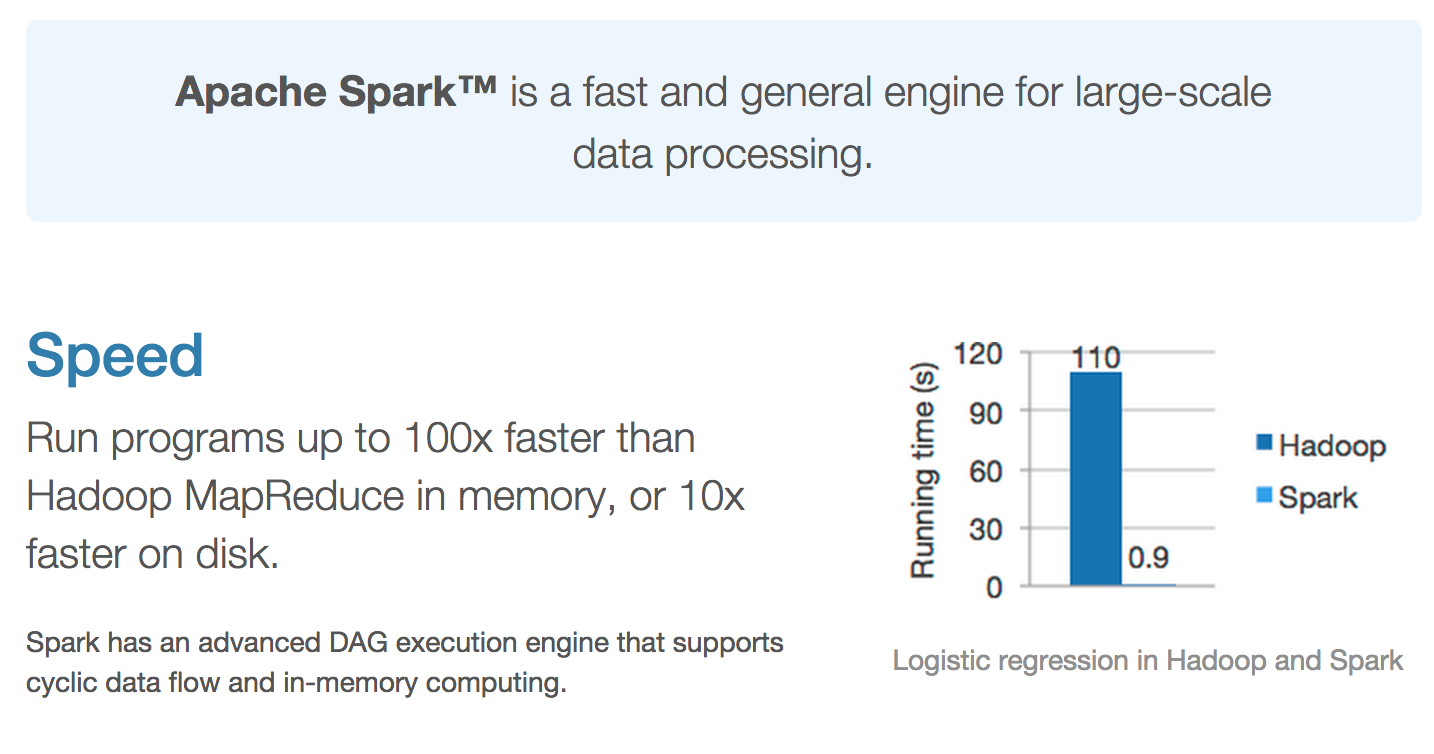
\includegraphics[width=0.8\textwidth]{spark.png}
  \end{center}
  \pause
  {\bf Problem:} Current performance studies do not show
  Spark's performance for interactive web analytics application.
}


\section{System Architecture}
\subsection{Mini-Project: Deploying Spark.}
\frame{\frametitle{\insertsection}
  \framesubtitle{
    \insertsubsection~\href{%
      http://github.com/adobe-research/spark-cluster-deployment}{%
      github/adobe-research/spark-cluster-deployment}}

  \begin{itemize}
    \item<+-> Spark is a trending distributed computing environment
      and favors in-memory processing.
    \item<+-> Documentation is currently biased towards writing
      Spark applications and does not provide best practices for
      running on a cluster.
    \item<+-> Spark provides 4 deployment modes: EC2, standalone, Mesos,
      and YARN.
    \item<+-> {\bf Motivation:} Spark's standalone cluster mode seems
      simplest to configure and use, but requires files to be synchronized
      across the cluster, including the Spark installation directory.
  \end{itemize} 
}

\frame{\frametitle{\insertsection}
  \framesubtitle{
    \insertsubsection~\href{%
      http://github.com/adobe-research/spark-cluster-deployment}{%
      github/adobe-research/spark-cluster-deployment}}

  \begin{itemize}\footnotesize
    \item<+-> \textit{Open source \textbf{Puppet} is a flexible, customizable
      framework available under the Apache 2.0 license designed to
      help system administrators automate the many repetitive tasks
      they regularly perform.}
    \item<+-> \textit{\textbf{Fabric} is a Python library and command-line
      tool for streamlining the use of SSH for application deployment
      or systems administration tasks.
    }
    \item<+-> Organizations have open-sourced Puppet projects for
      HDFS and Spark on GitHub to manage the server configurations.
    \item<+-> Use {\bf Fabric} to synchronize and deploy to the servers,
      which simplifies configuration changes by keeping
      all configuration locally.
  \end{itemize}
}

\frame{\frametitle{\insertsection}
  \framesubtitle{
    \insertsubsection~\href{%
      http://github.com/adobe-research/spark-cluster-deployment}{%
      github/adobe-research/spark-cluster-deployment}}

  \begin{center}
  \scalebox{0.5}{
  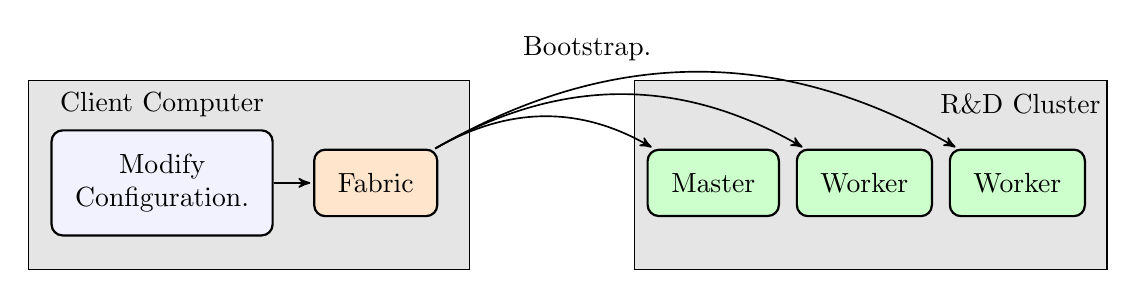
\begin{tikzpicture}
    \draw[fill=gray!20] (-1.7cm,-1.1cm) rectangle (3.9cm,1.3cm) {};
    \node[bn] (config) {Modify\\Configuration.};
    \node[on,right=0.5cm of config] (fabric) {Fabric};
    \node at (0cm,1cm) () {Client Computer};
    \draw[to] (config) -- (fabric);

    \draw[fill=gray!20] (6cm,-1.1cm) rectangle (12cm,1.3cm) {};
    \node[greenn] (m) at (7.0cm,0cm) {Master};
    \node[greenn,right=0.2cm of m] (w1) {Worker};
    \node[greenn,right=0.2cm of w1] (w2) {Worker};
    \node at (10.9cm,1cm) {R\&D Cluster};

    \node at (5.4cm,1.7cm) {Bootstrap.};
    \draw[to] (fabric) edge [bend left] (m);
    \draw[to] (fabric) edge [bend left] (w1);
    \draw[to] (fabric) edge [bend left] (w2);
  \end{tikzpicture}
  }
  \pause
  \scalebox{0.5}{
  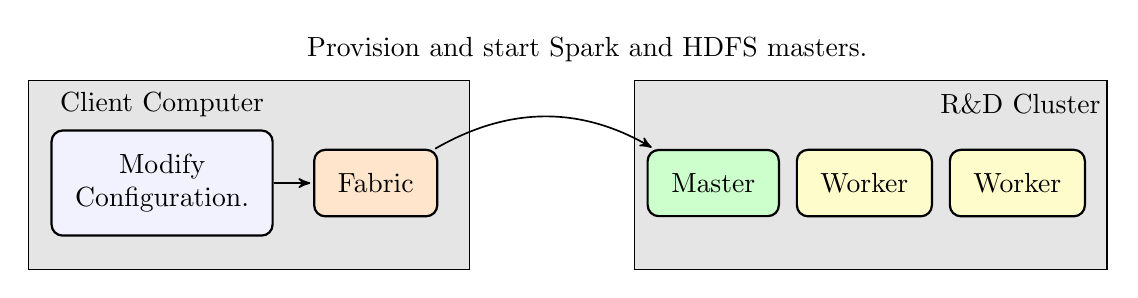
\begin{tikzpicture}
    \draw[fill=gray!20] (-1.7cm,-1.1cm) rectangle (3.9cm,1.3cm) {};
    \node[bn] (config) {Modify\\Configuration.};
    \node[on,right=0.5cm of config] (fabric) {Fabric};
    \node at (0cm,1cm) () {Client Computer};
    \draw[to] (config) -- (fabric);

    \draw[fill=gray!20] (6cm,-1.1cm) rectangle (12cm,1.3cm) {};
    \node[greenn] (m) at (7.0cm,0cm) {Master};
    \node[yn,right=0.2cm of m] (w1) {Worker};
    \node[yn,right=0.2cm of w1] (w2) {Worker};
    \node at (10.9cm,1cm) {R\&D Cluster};

    \node at (5.4cm,1.7cm) {Provision and start Spark and HDFS masters.};
    \draw[to] (fabric) edge [bend left] (m);
  \end{tikzpicture}
  }
  \pause
  \scalebox{0.5}{
  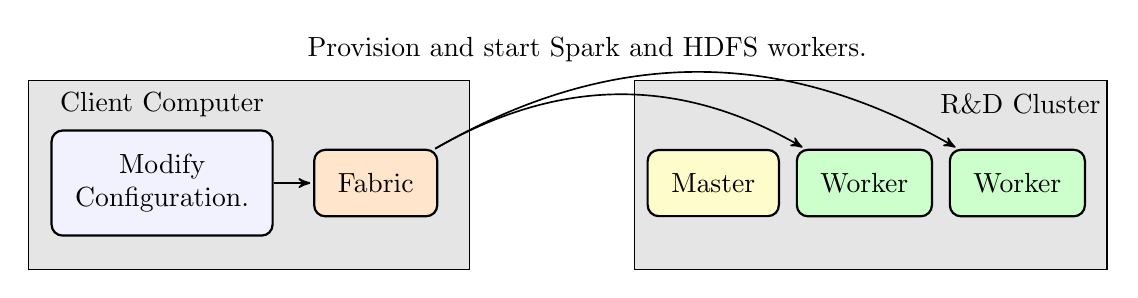
\begin{tikzpicture}
    \draw[fill=gray!20] (-1.7cm,-1.1cm) rectangle (3.9cm,1.3cm) {};
    \node[bn] (config) {Modify\\Configuration.};
    \node[on,right=0.5cm of config] (fabric) {Fabric};
    \node at (0cm,1cm) () {Client Computer};
    \draw[to] (config) -- (fabric);

    \draw[fill=gray!20] (6cm,-1.1cm) rectangle (12cm,1.3cm) {};
    \node[yn] (m) at (7.0cm,0cm) {Master};
    \node[greenn,right=0.2cm of m] (w1) {Worker};
    \node[greenn,right=0.2cm of w1] (w2) {Worker};
    \node at (10.9cm,1cm) {R\&D Cluster};

    \node at (5.4cm,1.7cm) {Provision and start Spark and HDFS workers.};
    \draw[to] (fabric) edge [bend left] (w1);
    \draw[to] (fabric) edge [bend left] (w2);
  \end{tikzpicture}
  }
  \end{center}
}

\frame{\frametitle{\insertsection}
  \framesubtitle{
    \insertsubsection~\href{%
      http://github.com/adobe-research/spark-cluster-deployment}{%
      github/adobe-research/spark-cluster-deployment}}

  \begin{itemize}\footnotesize
    \item<+-> {\bf Problem:} Deploying applications to a Spark cluster:
      \begin{itemize}
        \item<+-> Application JAR files need to be synchronized across every
          node on the cluster.
        \item<+-> Does not provide a way to obtain application output.
      \end{itemize}
    \item<+-> {\bf Solution:} Utilize Fabric to deploy, get output,
      and kill jobs on a Spark cluster.
  \end{itemize}
  \bigskip
  \pause
  \begin{center}
  \scalebox{0.6}{
  \begin{tikzpicture}
    \draw[fill=gray!20] (-2.5cm,-0.7cm) rectangle (5.6cm,2.2cm) {};
    \node at (4.5,1.1) (mac) {
\includegraphics[width=2cm]{mac.png}};
    \node at (4.2cm, 1.9cm) {{Client Computer}};
    \node[bn] (sbt) {sbt};
    \node[on,above left=0.5cm and -0.5cm of sbt] (lib) {Libraries};
    \node[on,above right=0.5cm and -0.5cm of sbt] (src) {Scala Sources};

    \draw[to] (lib) -- (sbt);
    \draw[to] (src) -- (sbt);

    \node[rn,right=of sbt] (jar) {Jar};
    \draw[to] (sbt) -- (jar);

    \node[yn,right=of jar] (fab) {Fabric};
    \draw[to] (jar) -- (fab);

    \node[below left=of fab] (s1) {};
    \node[below=of fab] (s2) {};
    \node[below right=of fab] (s3) {};
    \node[below=of fab] (spark) {Spark master and workers.};

    \draw[to] (fab) -- (s1);
    \draw[to] (fab) -- (s2);
    \draw[to] (fab) -- (s3);
  \end{tikzpicture}
  }
  \end{center}
}

\subsection{Requests and responses with Spray.}
\frame{\frametitle{\insertsection}\framesubtitle{\insertsubsection}
  {\bf Motivation:} How can we use expose our analytics engine to other
  components of Adobe's infrastructure?
  \pause
  \begin{center}
    
\includegraphics[height=1.5cm]{images/spray.png}
  \end{center}
  \pause
  {\bf Solution:} \textit{\textbf{spray} is an open-source toolkit for building
    REST/HTTP-based integration layers on top of Scala and Akka Actors.
    Being asynchronous, actor-based, fast, lightweight, modular and
    testable it's a great way to connect your Scala applications to the world.
  }
}

\frame{\frametitle{\insertsection}\framesubtitle{\insertsubsection}
  \begin{center}
  \scalebox{0.65}{
  \begin{tikzpicture}
    \node[bn] (query) {{\tt http://server/query}};
    \pause

    \node[greenn,right=of query] (spray) {
      
\includegraphics[height=.3cm]{images/spray.png}
    };
    \node at (1.9cm,1.1cm) {{\footnotesize HTTP Request}};
    \node at (1.7cm,-1.2cm)
      {{\footnotesize HTTP Response}\\{\footnotesize (HTML or text)}};
    \draw[to] (query) edge [bend left] (spray);
    \draw[to] (spray) edge [bend left] (query);
    \pause

    \draw[squig] (3.4cm,-0.6cm) -- (3.4cm,-1.5cm);
    \draw[squig] (3.9cm,-0.6cm) -- (3.9cm,-1.5cm);
    \draw[squig] (4.4cm,-0.6cm) -- (4.4cm,-1.5cm);
    \pause

    \draw[fill=yellow!20] (4.2cm,-1.6cm) rectangle (4.6cm,-0.5cm) {};
    \draw[squig] (4.4cm,-0.6cm) -- (4.4cm,-1.5cm);
    \pause

    \node[yn,right=of spray] (queryservice) {QueryService Actor};
    \node at (5.5cm,1.1cm) {{\footnotesize Spray Request}};
    \node at (5.7cm,-1.2cm) {{\footnotesize Spray Response} \\
      {\footnotesize (Future)}};
    \draw[to] (spray) edge [bend left] (queryservice);
    \draw[to] (queryservice) edge [bend left] (spray);
    \pause

    \node[yn,right=of queryservice] (queryprocessor) {QueryProcessor};
    \draw[to] (queryservice) edge [bend left] (queryprocessor);
    \draw[to] (queryprocessor) edge [bend left] (queryservice);
    \pause

    \node[rn,above=of queryprocessor] (sc)
      {{\footnotesize Global Spark Context}};
    \draw[tofrom] (queryprocessor) -- (sc);
    \pause

    \node[grayn,below=of queryprocessor] (db)
      {{\footnotesize HDFS/Parquet/Thrift}};
    \draw[tofrom] (queryprocessor) -- (db);
  \end{tikzpicture}
  }
  \end{center}
}

\subsection{Mini-Project: Columnar data store.}
\frame{\frametitle{\insertsection}
  \framesubtitle{
    \insertsubsection~\href{%
      http://github.com/adobe-research/spark-parquet-thrift-example}{%
      github/adobe-research/spark-parquet-thrift-example}}
  \begin{itemize}
    \item<+-> {\bf Motivation:} Adobe's web analytics data is sparse and has
      approximately 250 columns, and
      queries implemented in Spindle use less than ten columns.
    \item<+-> {\bf Solution:} Store the data in columnar store
      databases separated by day with {\bf Thrift} and
      {\bf Parquet} on {\bf HDFS}.
  \end{itemize}
}

\frame{\frametitle{\insertsection}
  \framesubtitle{
    \insertsubsection~\href{%
      http://github.com/adobe-research/spark-parquet-thrift-example}{%
      github/adobe-research/spark-parquet-thrift-example}}
  \begin{itemize}
    \item<+-> \textit{\textbf{Apache Thrift} allows you to define data
      types and service interfaces
      in a simple definition file. Taking that file as input, the compiler
      generates code to be used to easily build RPC clients and servers that
      communicate seamlessly across programming languages.
    }
    \item<+-> \textit{We created \textbf{Parquet} to make the advantages of
      compressed, efficient columnar data representation available to any
      project in the Hadoop ecosystem, regardless of the choice of data
      processing framework, data model, or programming language.
    }
  \end{itemize}
}

\frame{\frametitle{\insertsection}
  \framesubtitle{
    \insertsubsection~\href{%
      http://github.com/adobe-research/spark-parquet-thrift-example}{%
      github/adobe-research/spark-parquet-thrift-example}}
  \begin{itemize}
    \item<+-> Load each day into a Parquet database on HDFS.
      \begin{center}
      \scalebox{0.7}{
      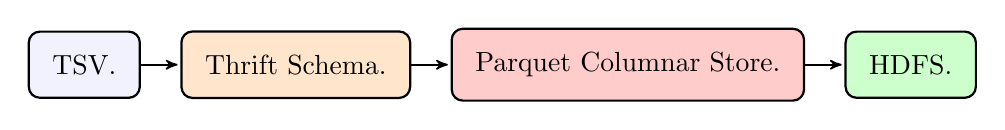
\begin{tikzpicture}
        \node[bn] (a) {TSV.};
        \node[on,right=0.5cm of a] (b) {Thrift Schema.};
        \node[rn,right=0.5cm of b] (c) {Parquet Columnar Store.};
        \node[greenn,right=0.5cm of c] (d) {HDFS.};
        \draw[to] (a) -- (b);
        \draw[to] (b) -- (c);
        \draw[to] (c) -- (d);
      \end{tikzpicture}
      }
      \end{center}
    \item<+-> Retrieve data by specifying column subsets.
      \begin{center}
      \scalebox{0.7}{
      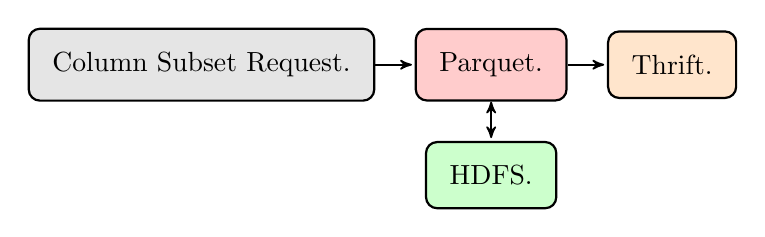
\begin{tikzpicture}
        \node[grayn] (a) {Column Subset Request.};
        \node[rn,right=0.5cm of a] (b) {Parquet.};
        \node[on,right=0.5cm of b] (c) {Thrift.};
        \node[greenn,below=0.5cm of b] (d) {HDFS.};
        \draw[to] (a) -- (b);
        \draw[to] (b) -- (c);
        \draw[tofrom] (b) -- (d);
      \end{tikzpicture}
      }
      \end{center}
  \end{itemize}
}

\frame{\frametitle{\insertsection}\framesubtitle{\insertsubsection}
  \begin{itemize}
    \item<+-> Load RDD's into a Scala {\tt Seq}.
    \item<+-> Only works well for a single timezone of data.
  \end{itemize}
  \begin{center}
  \scalebox{0.7}{
  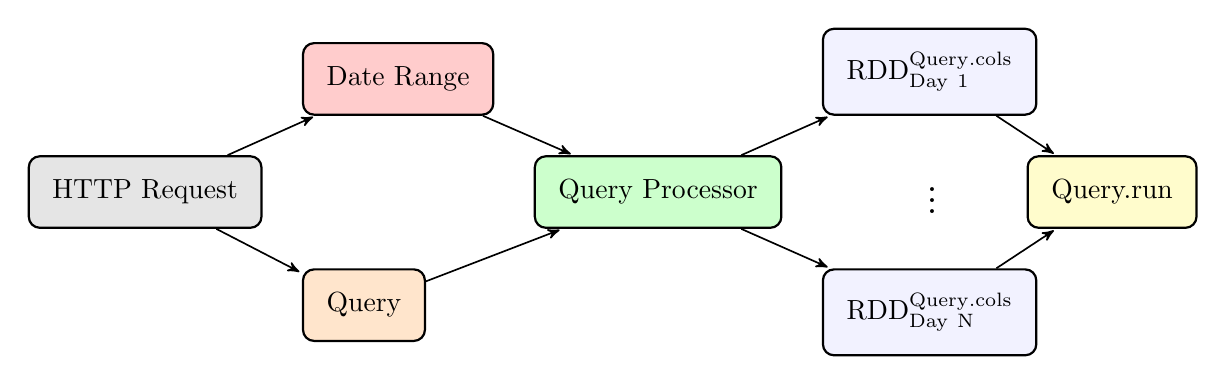
\begin{tikzpicture}
    \node[grayn] (a) {HTTP Request};
    \node[rn,above right=0.5cm and 0.5cm of a] (b) {Date Range};
    \node[on,below right=0.5cm and 0.5cm of a] (c) {Query};
    \node[greenn,below right=0.5cm and 0.5cm of b] (d) {Query Processor};
    \node[bn,above right=0.5cm and 0.5cm of d] (e)
      {RDD$_{\rm Day~1}^{\rm Query.cols}$};
    \node[bn,below right=0.5cm and 0.5cm of d] (f)
      {RDD$_{\rm Day~N}^{\rm Query.cols}$};
    \node[right=1.7cm of d] (g) {{\LARGE $\vdots$}};
    \node[yn,right=of g] (h) {Query.run};
    \draw[to] (a) -- (b); \draw[to] (a) -- (c); \draw[to] (b) -- (d);
    \draw[to] (c) -- (d); \draw[to] (d) -- (e); \draw[to] (d) -- (f);
    \draw[to] (e) -- (h); \draw[to] (f) -- (h);
  \end{tikzpicture}
  }
  \end{center}
}

\subsection{Simple caching policy.}
\frame{\frametitle{\insertsection}\framesubtitle{\insertsubsection}
  \begin{itemize}
    \item<+-> {\bf Motivation:} Loading gigabytes or terabytes of data
      is a performance bottleneck for many applications, and
      web analytics queries are likely to be on the same data set.
    \item<+-> {\bf Possible Solution:}
      \textit{\textbf{Tachyon} is a memory-centric distributed
      file system that runs on top of HDFS and caches working
      set files in memory.
      Tachyon is Hadoop compatible and can be used with Spark or
      MapReduce programs without any code change.
    }
  \end{itemize}
}

\frame{\frametitle{\insertsection}\framesubtitle{\insertsubsection}
  \begin{center}
  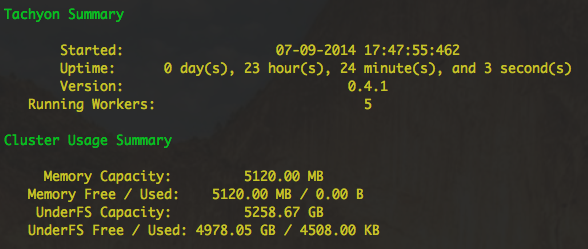
\includegraphics[width=0.7\textwidth]{tachyon-3.png}
  \end{center}
  \pause
  \begin{itemize}
    \item<+-> Parquet optimizes disk accesses and only reads specific blocks
      while loading files and never entire file.
      However, Tachyon 0.4.1 cannot cache random file block accesses
      and has the severe limitation of only caching files
      when all blocks are read.
    \item<+-> Confirmed by emailing Tachyon's mailing list.
  \end{itemize}
}

\frame{\frametitle{\insertsection}\framesubtitle{\insertsubsection}
  \begin{itemize}
    \item<+-> {\bf Workaround Solution:} Provide a {\tt cache} parameter
      that saves RDD's in memory between query calls.
    \item<+-> This works well for benchmarking single queries on the same data,
      but requires substantial engineering effort to make production-ready.
      \begin{itemize}
        \item<+-> Two queries could be submitted on the same date range that
          request overlapping, but not identical, column subsets.
          How should these data sets with partially overlapping values be
          cached?
        \item<+-> What if one of the queries is called substantially more times
          than the others?
          How can the caching policy recommend the data required by
          these queries be cached?
      \end{itemize}
  \end{itemize}
}

\frame{\frametitle{\insertsection}\framesubtitle{\insertsubsection}
  \begin{center}
  \scalebox{0.7}{
  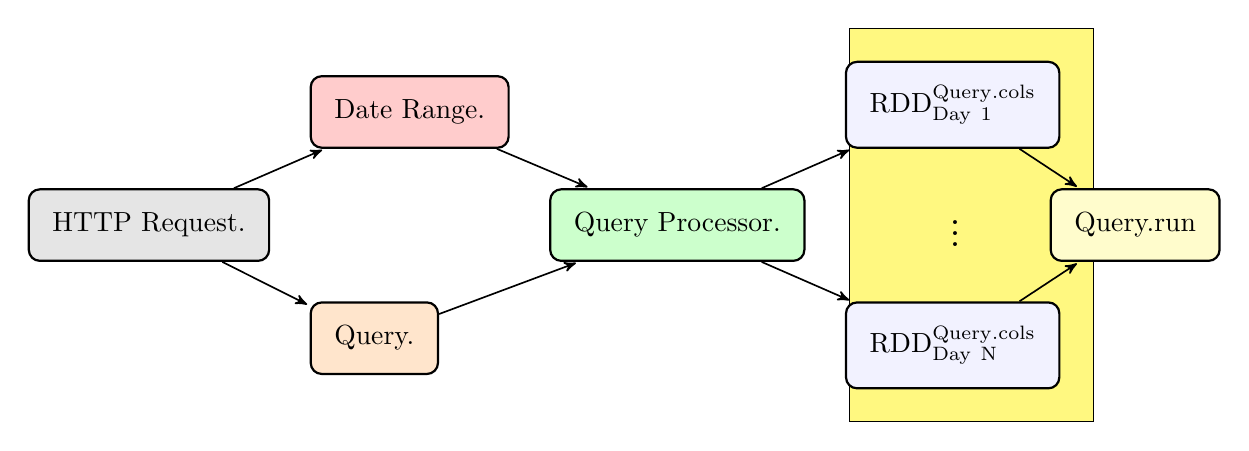
\begin{tikzpicture}
    \draw[fill=yellow!50] (8.9,-2.5) rectangle (12,2.5);
    \node[grayn] (a) {HTTP Request.};
    \node[rn,above right=0.5cm and 0.5cm of a] (b) {Date Range.};
    \node[on,below right=0.5cm and 0.5cm of a] (c) {Query.};
    \node[greenn,below right=0.5cm and 0.5cm of b] (d) {Query Processor.};
    \node[bn,above right=0.5cm and 0.5cm of d] (e)
      {RDD$_{\rm Day~1}^{\rm Query.cols}$};
    \node[bn,below right=0.5cm and 0.5cm of d] (f)
      {RDD$_{\rm Day~N}^{\rm Query.cols}$};
    \node[right=1.7cm of d] (g) {{\LARGE $\vdots$}};
    \node[yn,right=of g] (h) {Query.run};
    \draw[to] (a) -- (b); \draw[to] (a) -- (c); \draw[to] (b) -- (d);
    \draw[to] (c) -- (d); \draw[to] (d) -- (e); \draw[to] (d) -- (f);
    \draw[to] (e) -- (h); \draw[to] (f) -- (h);
  \end{tikzpicture}
  }
  \end{center}
}

\iffalse
\subsection{Partitioning.}
\frame{\frametitle{\insertsection}\framesubtitle{\insertsubsection}
  \begin{itemize}
    \item<+-> Spark provides an option to some operations to specify how tasks
      are partitioned across nodes.
    \item<+-> Partitioning when loading data is a common option, but is
      currently undocumented for Spark and Parquet.
    \item<+-> However, other operations such as distinct, reducebyKey,
      and groupByKey provide an optional argument to specify
      the minimum number of resulting partitions.
  \end{itemize}
}

\frame{\frametitle{\insertsection}\framesubtitle{\insertsubsection}
  \begin{itemize}
    \item<+-> Counting the number of records in a Spark intermediate form is
      expensive, and automatically knowing the optimal number of partitions
      for operations depends highly on the data and operations.
    \item<+->  Spindle attempts to put a target number of records in each partition
      by estimating the total number of records to be processed
      from Parquet's metadata.
    \item<+-> However, web analytics data is sparse and most queries filter
      records before doing operations that impact the partitioning.
  \end{itemize}
}
\fi

\subsection{Queries.}
\newcommand{\nameMapsRow}[2]{#2 & #1 \\}
\newcommand{\mt}{\ensuremath{\times}}
\frame{\frametitle{\insertsection}
  \framesubtitle{\insertsubsection~Demo at \url{http://adobe-research.github.io/spindle}}
\begin{table}[hb]
  \centering
  \tiny
  \begin{tabular}{rl}
    Shorthand & Name \\ \hline
    \nameMapsRow{Pageviews}{Q0}
    \nameMapsRow{Revenue}{Q1}
    \nameMapsRow{RevenueFromTopReferringDomains}{Q2}
    \nameMapsRow{RevenueFromTopReferringDomainsFirstVisitGoogle}{Q3}
    \nameMapsRow{TopPages}{Q4}
    \nameMapsRow{TopPagesByBrowser}{Q5}
    \nameMapsRow{TopPagesByPreviousTopPages}{Q6}
    \nameMapsRow{TopReferringDomains}{Q7}
  \end{tabular}
\end{table}
\bigskip
\pause
\begin{table}[ht]
  \centering
  \tiny
  \begin{tabular}{ccccccccc}
  &
    Q0 &  Q1  &  Q2  &  Q3  &  Q4  &  Q5  &  Q6  &  Q7  \\ \hline
  post\_pagename &
   \mt &      &      &      &  \mt &  \mt &  \mt &      \\
  user\_agent &
       &      &      &      &      &  \mt &      &      \\
  visit\_referrer &
       &      &  \mt &  \mt &      &      &      &      \\
  post\_visid\_high &
       &      &  \mt &  \mt &      &      &  \mt &  \mt \\
  post\_visid\_low &
       &      &  \mt &  \mt &      &      &  \mt &  \mt \\
  visit\_num &
       &      &  \mt &  \mt &      &      &  \mt &  \mt \\
  visit\_referrer &
       &      &      &      &      &      &      &  \mt \\
  hit\_time\_gmt &
       &      &      &      &      &      &  \mt &      \\
  post\_purchaseid &
       &  \mt &  \mt &  \mt &      &      &      &      \\
  post\_product\_list &
       &  \mt &  \mt &  \mt &      &      &      &      \\
  first\_hit\_referrer &
       &      &      &  \mt &      &      &      &      \\
  \end{tabular}
\end{table}
}

\iffalse
\newcommand{\queryOpRow}[2]{#1 & #2 \\}
\frame{\frametitle{\insertsection}
  \framesubtitle{\insertsubsection~Demo at \url{http://adobe-research.github.io/spindle}}
  \begin{itemize}
    \item<+-> Table below shows high-level Spark operations.
    \item<+-> Italicized operations indicate operations where partitioning is
      specified.
  \end{itemize}
  \bigskip
  \begin{table}[hb]
    \centering
    \tiny
    \begin{tabular}{@{}l@{\hskip 1mm}l@{}}
      Query & Operations \\ \hline
      \queryOpRow{Q0}{map$\rightarrow$count}
      \queryOpRow{Q1}{collect$\rightarrow$reduce}
      \queryOpRow{Q2}{collect$\rightarrow${\it distinct}$\rightarrow$collect$\rightarrow${\it reduceByKey}$\rightarrow$top$\rightarrow$collect$\rightarrow$reduce}
      \queryOpRow{Q3}{collect$\rightarrow${\it distinct}$\rightarrow$collect$\rightarrow${\it reduceByKey}$\rightarrow$top$\rightarrow$collect$\rightarrow$reduce}
      \queryOpRow{Q4}{collect$\rightarrow${\it reduceByKey}$\rightarrow$top}
      \queryOpRow{Q5}{collect$\rightarrow${\it reduceByKey}$\rightarrow$top$\rightarrow$collect$\rightarrow$reduceByKey$\rightarrow$top}
      \queryOpRow{Q6}{collect$\rightarrow${\it reduceByKey}$\rightarrow$top$\rightarrow$collect$\rightarrow${\it groupByKey}$\rightarrow$map$\rightarrow$reduceByKey$\rightarrow$top}
      \queryOpRow{Q7}{collect$\rightarrow${\it distinct}$\rightarrow$collect$\rightarrow${\it reduceByKey}$\rightarrow$top}
    \end{tabular}
  \end{table}
}
\fi

\begin{frame}[fragile]
  \frametitle{\insertsection}
  \framesubtitle{\insertsubsection~Demo at \url{http://adobe-research.github.io/spindle}}

  \begin{lstlisting}[language=scala]
case class QueryConf(
  sc: SparkContext, data: Array[RDD[SiteCatalyst]], profile: Boolean,
  daysInRange: Seq[String], dailyRows: Seq[Long], targetPartitionSize: Long
)|\pause|

object TopPages extends Query {|\pause|
  def colsNeeded = Seq("post_pagename")|\pause|
  def run(c: QueryConf) = {|\pause|
    val allData = c.sc.union(c.data); val numAllRows = c.dailyRows.reduce(_+_)
    val numPartitions = (numAllRows/c.targetPartitionSize).toInt|\pause|
    val queryResult = allData.collect{
        case (root) if !root.post_pagename.isEmpty => (root.post_pagename, 1)
      }|\pause|
      .reduceByKey(_+_,numPartitions)|\pause|
      .top(10) {
        Ordering.by((entry: ((String, Int))) => entry._2)
      }.toSeq|\pause|
    if (c.profile)
      "[" + queryResult.map("\"" + _.toString + "\"").mkString(", ") + "]"|\pause|
    else {
      html.TopPages("TopPages", c.daysInRange, queryResult).toString
    }
  }
}
  \end{lstlisting}
\end{frame}


\frame{\frametitle{\insertsection}
  \framesubtitle{\insertsubsection}
  \begin{center}
    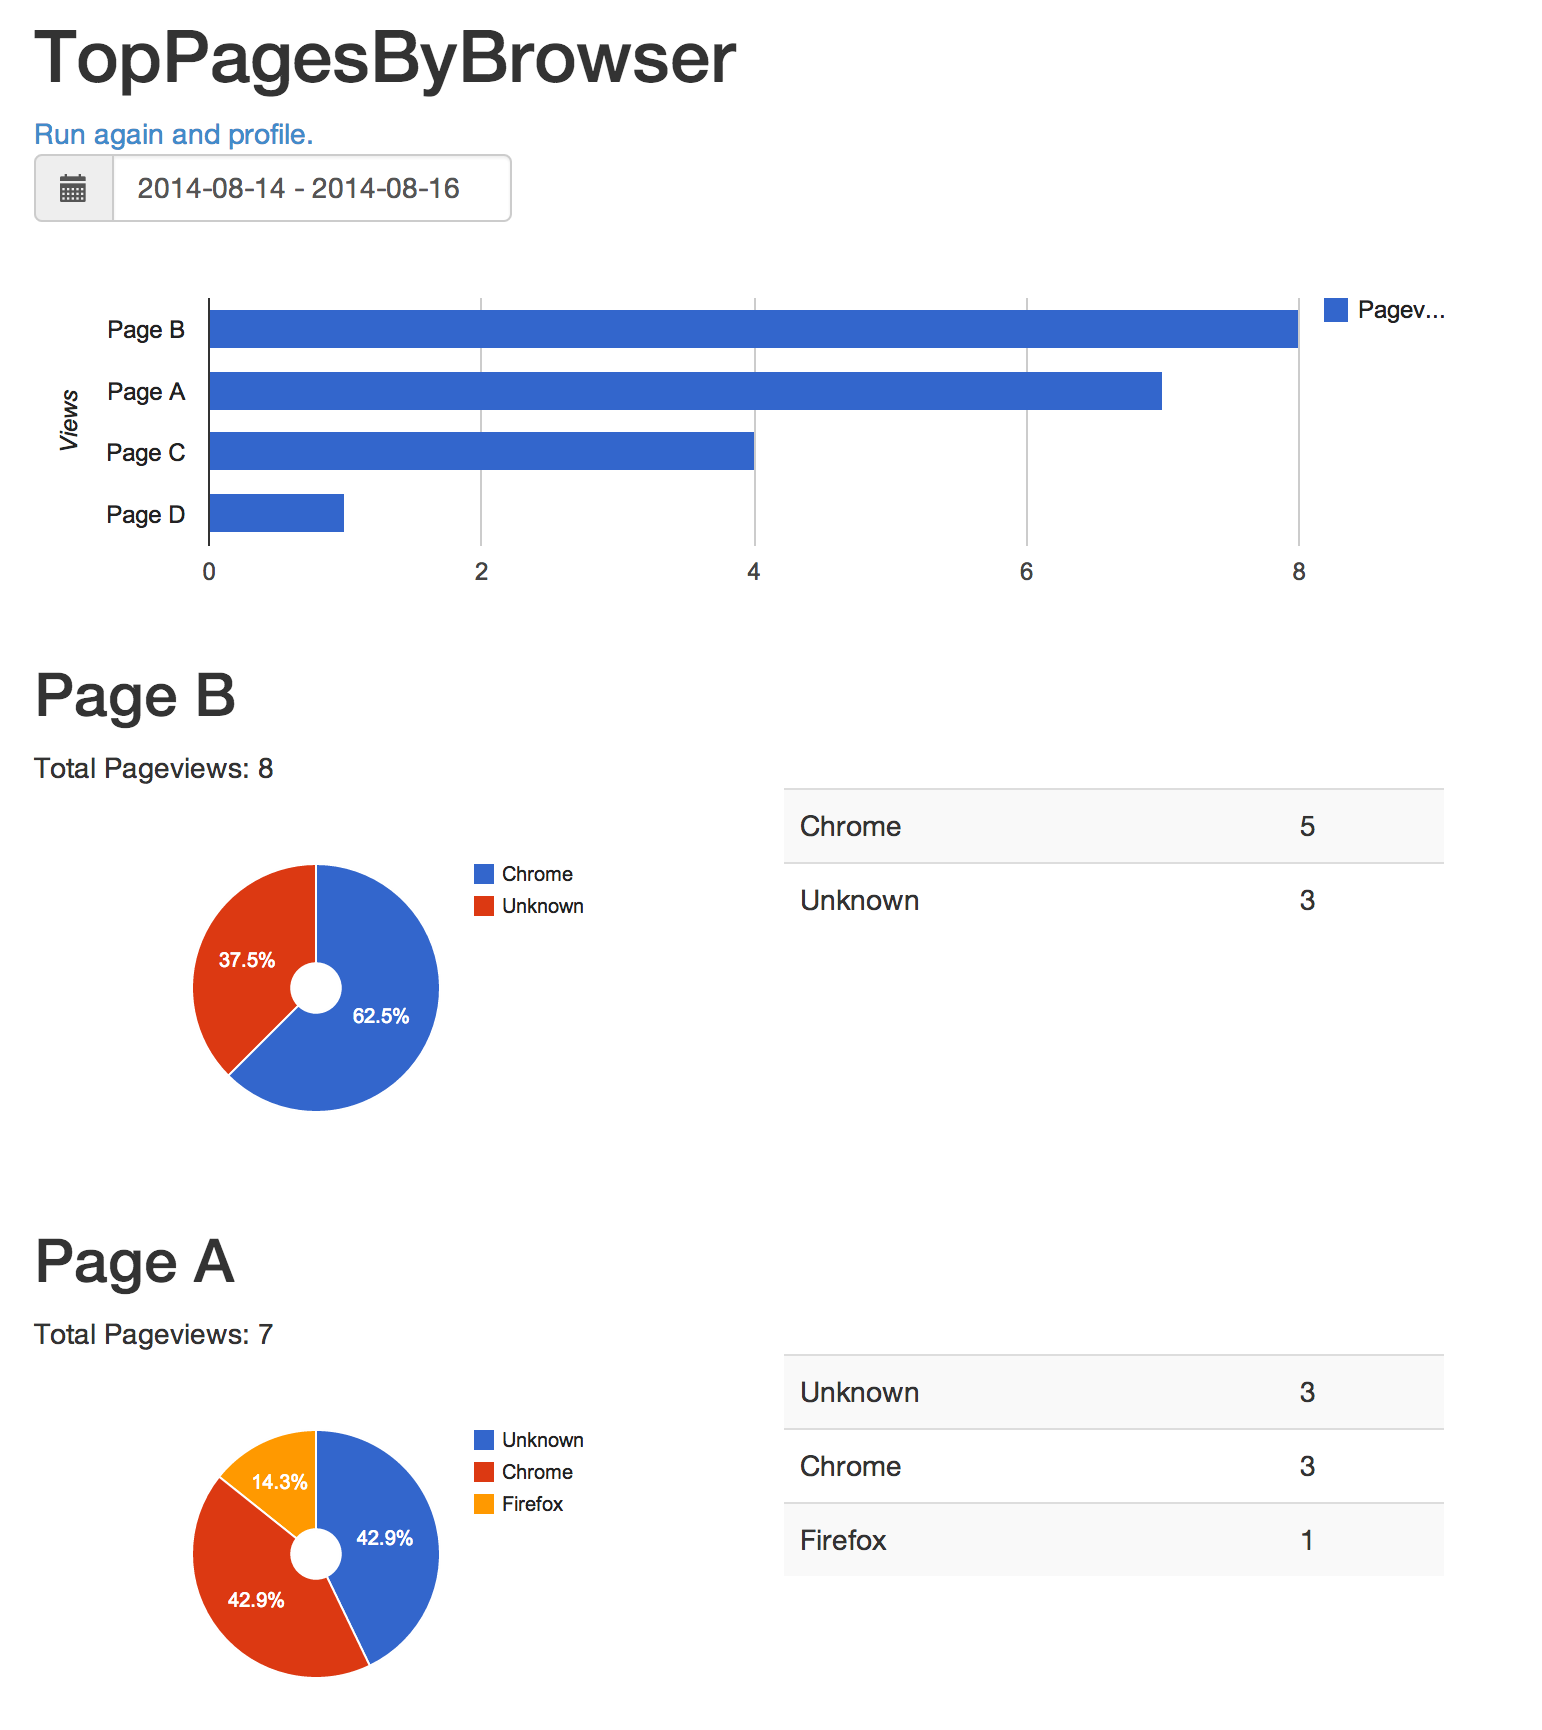
\includegraphics[width=0.8\textwidth]{top-pages-by-browser.png}
  \end{center}
}

\subsection{Ad hoc queries.}
\frame{\frametitle{\insertsection}\framesubtitle{\insertsubsection}
  \begin{itemize}
    \item<+-> Spark SQL is an alpha feature in Spark and allows
      relational queries in SQL to be executed with Spark.
    \item<+-> SiteCatalyst Parquet on HDFS can be loaded directly into
      the Spark SQL data types and queried with SQL strings.
  \end{itemize}
}

\frame{\frametitle{\insertsection}\framesubtitle{\insertsubsection}
  \begin{center}
    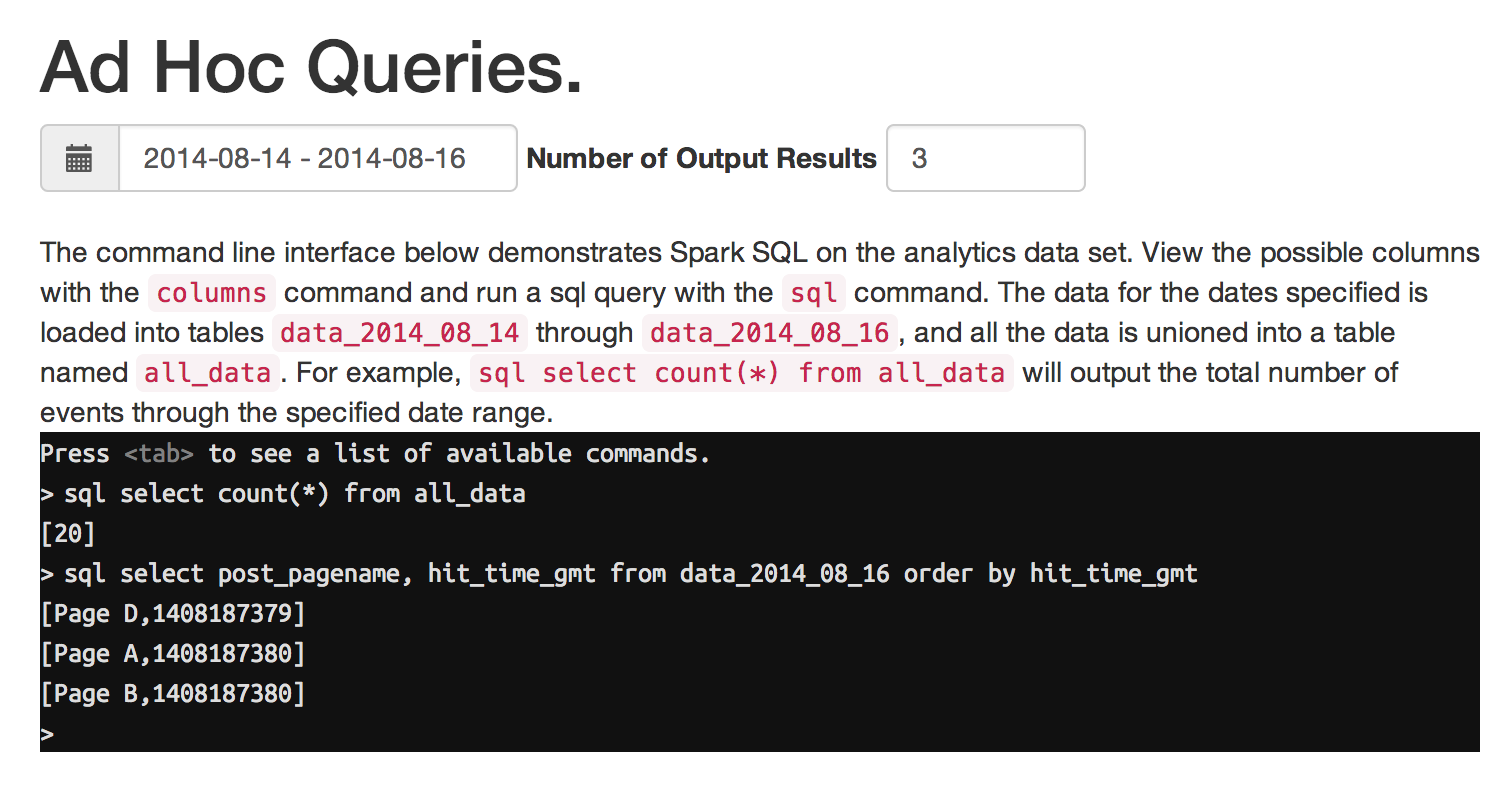
\includegraphics[width=0.9\textwidth]{adhoc.png}
  \end{center}
}

\section{Empirical Results}
\subsection{Experimental Data}
\frame{\frametitle{\insertsection}\framesubtitle{\insertsubsection}
  \begin{itemize}
    \item<+-> Query date range is Jan 1, 2014 to Jan 7, 2014, inclusively.
    \item<+-> Each Spark worker has 24 cores and 20GB of memory.
    \item<+-> The entire Parquet databases on HDFS for each day
      totals 13.1GB.
    %\item<+-> For partitioning, 49\% of records have empty
     % post\_pagename values, and 50.4\% of records have empty
     % visit\_referrer values.
    \item<+-> Benchmarking is done with a Python script, and plots
      are produced with pyplot.
  \end{itemize}
}

\iffalse
\frame{\frametitle{\insertsection}\framesubtitle{\insertsubsection}
  \begin{itemize}
    \item<+-> Because 6 workers are being used with 20GB of memory each,
      $\leq7$ columns into memory should never cause memory or
      paging issues.
  \end{itemize}
  \bigskip
  \begin{table}[ht]
    \centering\tiny
    \begin{tabular}{cc}
      Column & Gigabytes \\ \hline
      post\_pagename & 0.286 \\
      post\_visid\_high & 0.436 \\
      post\_visid\_low & 0.436 \\
      visit\_num & 0.029 \\
      hit\_time\_gmt & 0.230 \\
      visit\_referrer & 1.705 \\
      post\_purchaseid & 0.000356 \\
      post\_product\_list & 1.890 \\
      first\_hit\_referrer & 2.070 \\
    \end{tabular}
  \end{table}
}
\fi

\subsection{Ideal number of partitions.}
\frame{\frametitle{\insertsection}\framesubtitle{\insertsubsection}
  \begin{itemize}
    \item<+-> Using 6 workers, vary the target partition sizes for each
      query that uses partitioning.
    \item<+-> Don't cache data and sample each target partition size 4 times.
  \end{itemize}
}

\frame{\frametitle{\insertsection}\framesubtitle{\insertsubsection}
  \begin{figure}[ht]
    \centering
    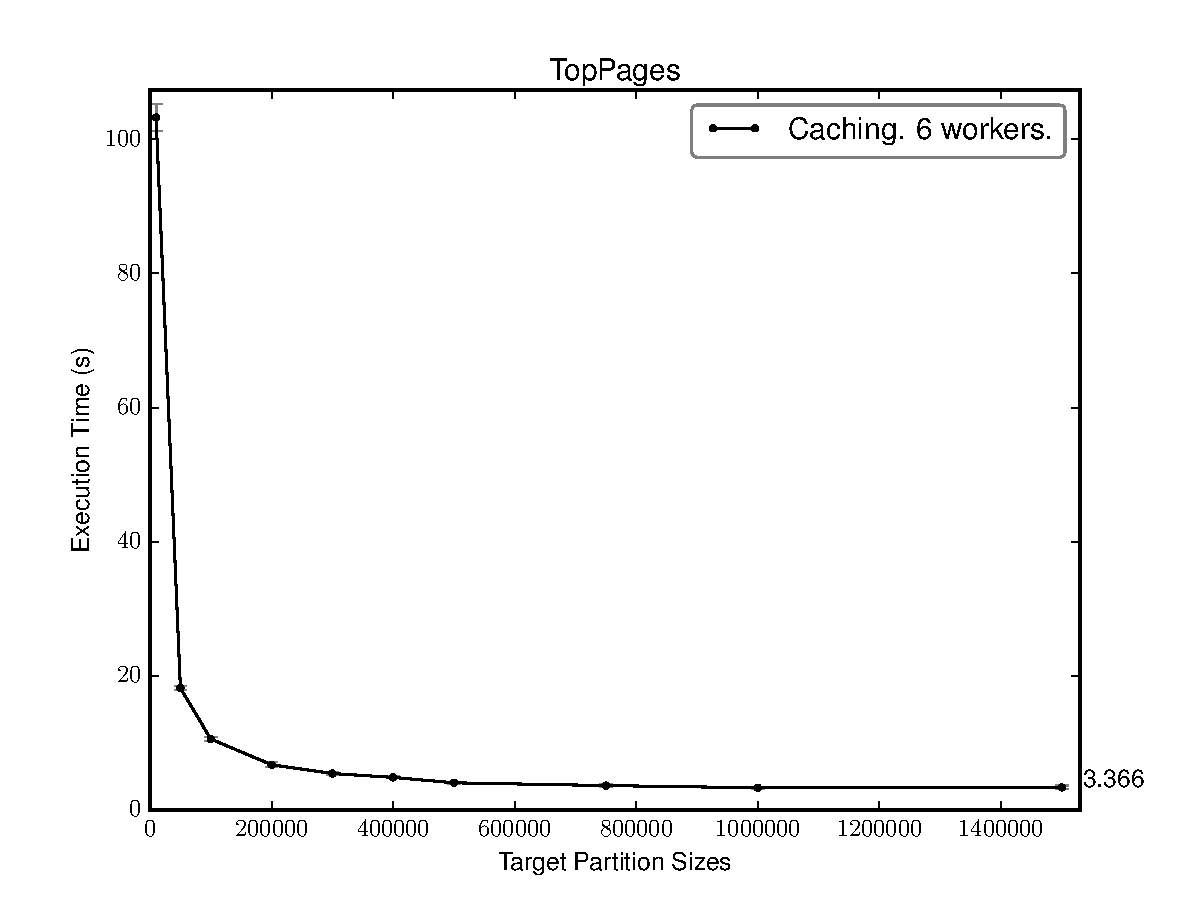
\includegraphics[width=0.7\textwidth]{results-2014.08.02/partitions/pdf/TopPages.pdf}
  \end{figure}
}

\frame{\frametitle{\insertsection}\framesubtitle{\insertsubsection}
  \begin{itemize}
    \item<+-> {\bf Conclusion:} Target 1.5M records in each partition for
      best performance on this data set.
  \end{itemize}
  \bigskip
  \begin{table}[ht]
    \centering\tiny
    \begin{tabular}{ccc}
      Query & Best Execution Time & Execution Time at 1.5M Target Size \\ \hline
      Q2 & 16853.50 & 16853.50 \\
      Q3 & 16934.25 & 16934.25 \\
      Q4 & 3241.25 & 3241.25 \\
      Q5 & 14862.00 & 14877.25 \\
      Q6 & 35554.50 & 37034.00 \\
      Q7 & 6597.25 & 6597.25 \\
    \end{tabular}
  \end{table}
}

\subsection{Caching.}
\frame{\frametitle{\insertsection}\framesubtitle{\insertsubsection}
  \begin{itemize}
    \item<+-> How much better performance does caching give?
    \item<+-> Leverage all 6 workers and target 1.5M records in each partition.
    \item<+-> Sample each point 4 times.
  \end{itemize}
}

\frame{\frametitle{\insertsection}\framesubtitle{\insertsubsection}
\begin{figure}[ht]
  \centering
  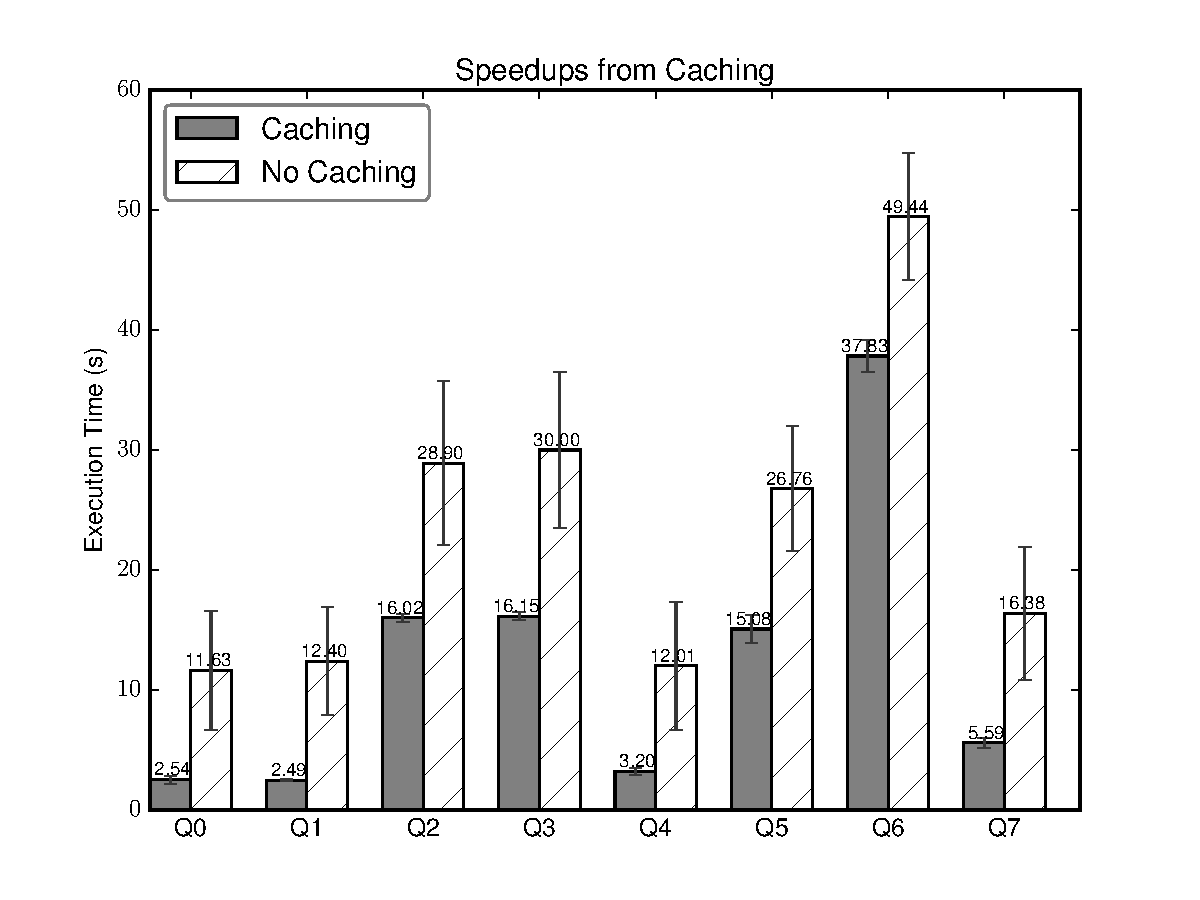
\includegraphics[width=0.7\textwidth]{results-2014.08.02/caching/caching.pdf}
\end{figure}
}

\subsection{Benchmarking concurrent queries.}
\frame{\frametitle{\insertsection}\framesubtitle{\insertsubsection}
  \begin{itemize}
    \item<+-> Multiple users can utilize an analytics system like SiteCatalyst
      concurrently, and Spark can be used in multithreaded applications.
    \item<+-> {\bf Research Question:} How much will Spark's performance
      degrade if multiple users are utilizing it at the same time?
    \item<+-> {\bf Solution:} Assume users submit the same query
      at the same time and observe the average query response time.
  \end{itemize}
}

\frame{\frametitle{\insertsection}\framesubtitle{\insertsubsection}
  \begin{itemize}
    \item<+-> A Python script using threading manages threads for
      each number of concurrent queries.
    \item<+-> Consider the example below for 2 threads and 3 repeated
      queries per thread. The first thread finishes before the second,
      and remains loaded until the second thread finishes.
      $t_4^1$ and $t_5^1$ are not used in the average.
    \item<+-> This experiment runs queries on the date range of
      Jan 1, 2014 to Jan 7, 2014 and each thread calls the query 4 times.
  \end{itemize}
  \begin{center}
  \scalebox{0.75}{
  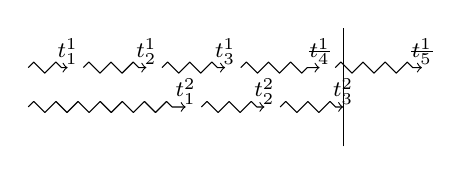
\begin{tikzpicture}
    \draw[squig] (0,0) -- (2,0);\node at (2,0.2) {{\footnotesize $t_1^2$}};
    \draw[squig] (2.2,0) -- (3,0);\node at (3,0.2) {{\footnotesize $t_2^2$}};
    \draw[squig] (3.2,0) -- (4,0);\node at (4,0.2) {{\footnotesize $t_3^2$}};

    \draw[squig] (0,0.5) -- (0.5,0.5);\node at (0.5,0.7)
      {{\footnotesize $t_1^1$}};
    \draw[squig] (0.7,0.5) -- (1.5,0.5);\node at (1.5,0.7)
      {{\footnotesize $t_2^1$}};
    \draw[squig] (1.7,0.5) -- (2.5,0.5);\node at (2.5,0.7)
      {{\footnotesize $t_3^1$}};
    \draw[squig] (2.7,0.5) -- (3.7,0.5);\node at (3.7,0.7)
      {{\footnotesize \sout{$t_4^1$}}};
    \draw[squig] (3.9,0.5) -- (5.0,0.5);\node at (5.0,0.7)
      {{\footnotesize \sout{$t_5^1$}}};

    \draw (4,-0.5) -- (4,1);
  \end{tikzpicture}
  }
  \end{center}
}

\frame{\frametitle{\insertsection}\framesubtitle{\insertsubsection}
  \begin{itemize}
    \item<+-> Speedups for all queries are similar to the following.
  \end{itemize}
  \bigskip
  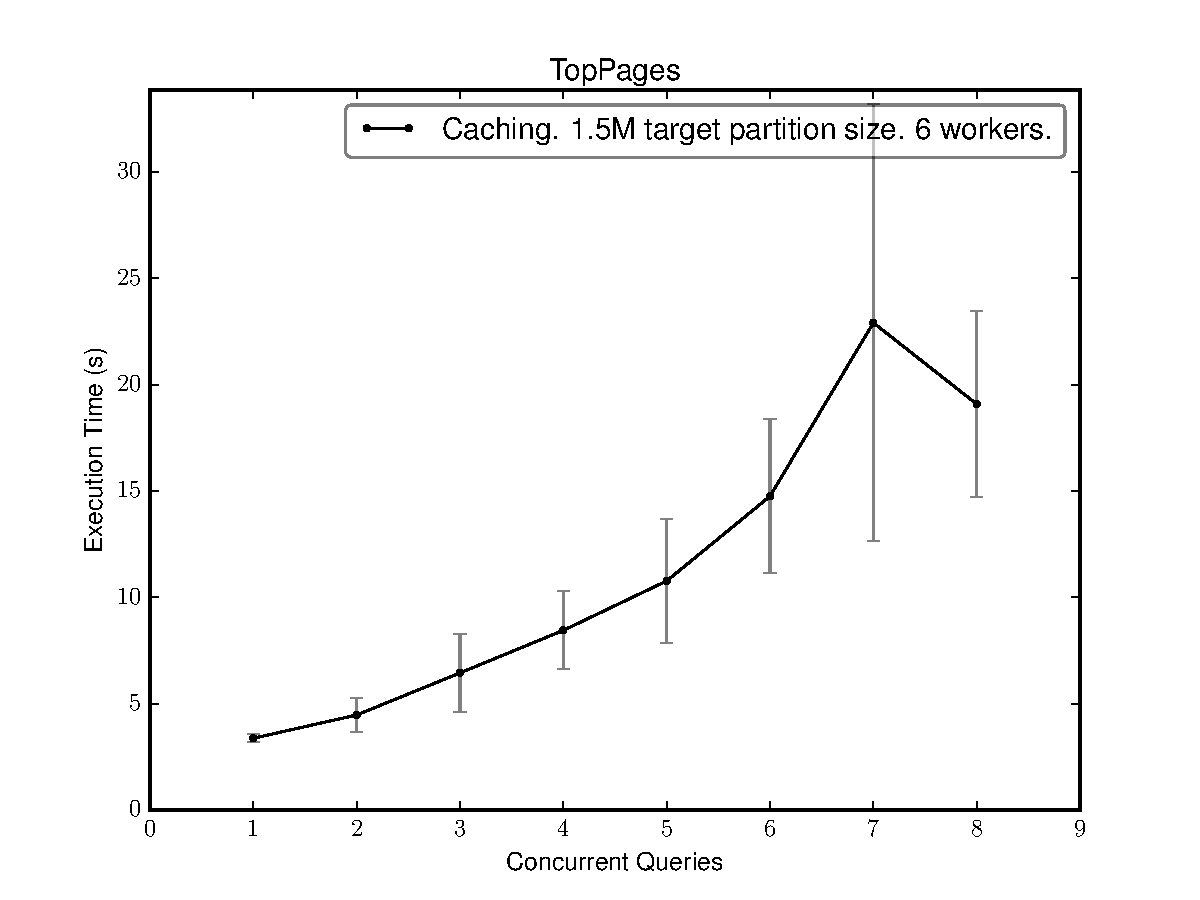
\includegraphics[width=0.5\textwidth]{results-2014.08.02/concurrent/pdf/TopPages.pdf}
  \pause
  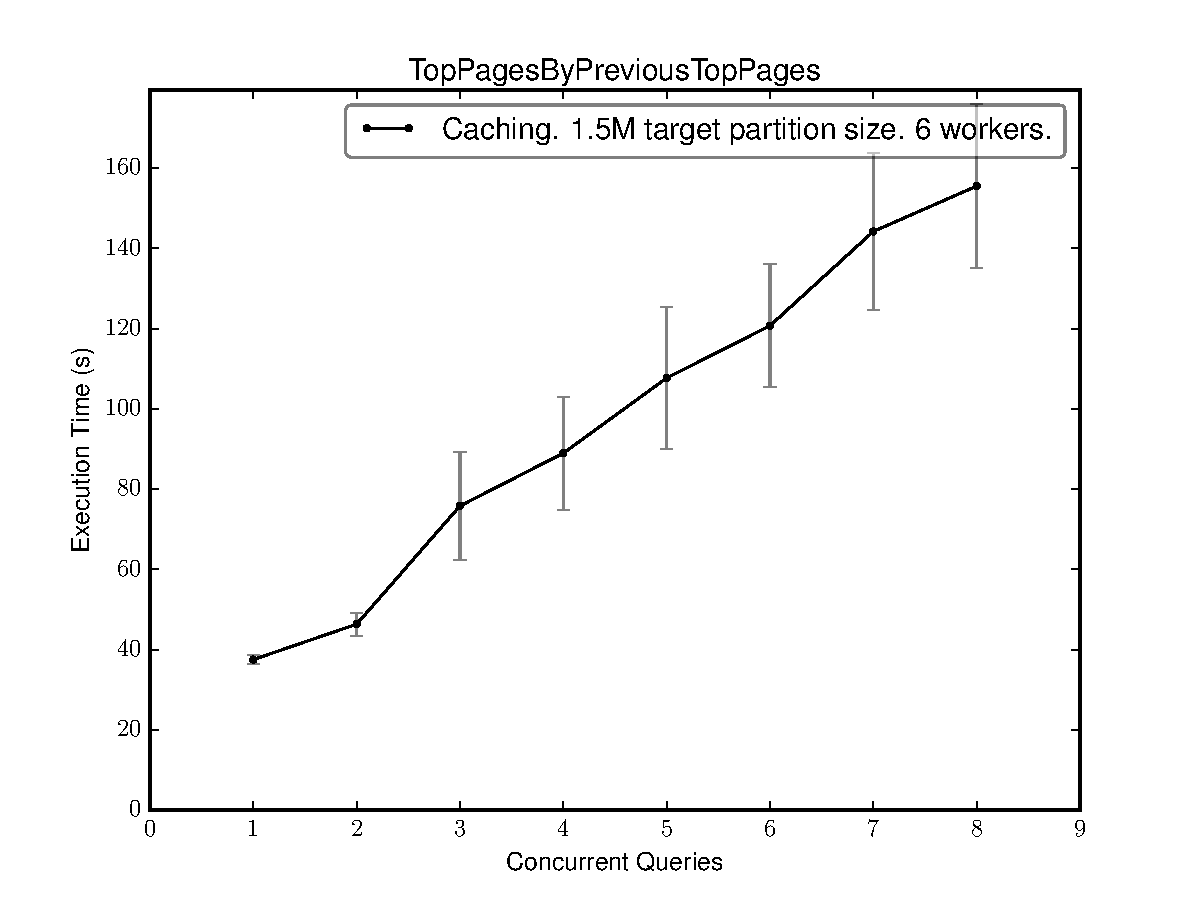
\includegraphics[width=0.5\textwidth]{results-2014.08.02/concurrent/pdf/TopPagesByPreviousTopPages.pdf}
}

\iffalse
\frame{\frametitle{\insertsection}\framesubtitle{\insertsubsection}
  \begin{itemize}
    \item<+-> {\bf Conclusion:} 6 workers don't scale well to 8 queries,
      but utilizing more workers should increase performance.
  \end{itemize}
  \bigskip
  \begin{table}[ht]
    \centering\tiny
    \begin{tabular}{cccc}
      Query & Serial Time (ms) & 2 Concurrent Slowdown &
        8 Concurrent Slowdown \\ \hline
      Q0 & 2420.75 & 1.69 & 6.41 \\
      Q1 & 2472.75 & 1.72 & 6.59 \\
      Q2 & 17052.25 & 1.70 & 6.60 \\
      Q3 & 16911.25 & 1.69 & 6.64 \\
      Q4 & 3256.50 & 1.38 & 5.19 \\
      Q5 & 15152.50 & 2.39 & 7.19 \\
      Q6 & 37529.25 & 1.66 & 4.28 \\
      Q7 & 6490.25 & 1.19 & 4.09 \\
    \end{tabular}
  \end{table}
}
\fi

\section{Conclusions}
\frame{\frametitle{\insertsection}\framesubtitle{\insertsubsection}
  \begin{itemize}
    \item<+-> Spark is a good candidate for real-time analytics processing.
    \item<+-> Spindle is a research prototype and benchmarkable analytics
      engine.
    \item<+-> Spindle's future work is on caching and preprocessing data.
  \end{itemize}
}

\frame{\frametitle{Questions?}
  \begin{center}
    {\scriptsize
      \begin{tabular}{r|l}
      {\bf Spindle Project} & \url{http://github.com/adobe-research/spindle} \\
      {\bf Brandon Amos} & \url{http://github.com/bamos} \\
      {\bf David Tompkins} & \url{http://github.com/DavidTompkins} \\
      \end{tabular}
    }
    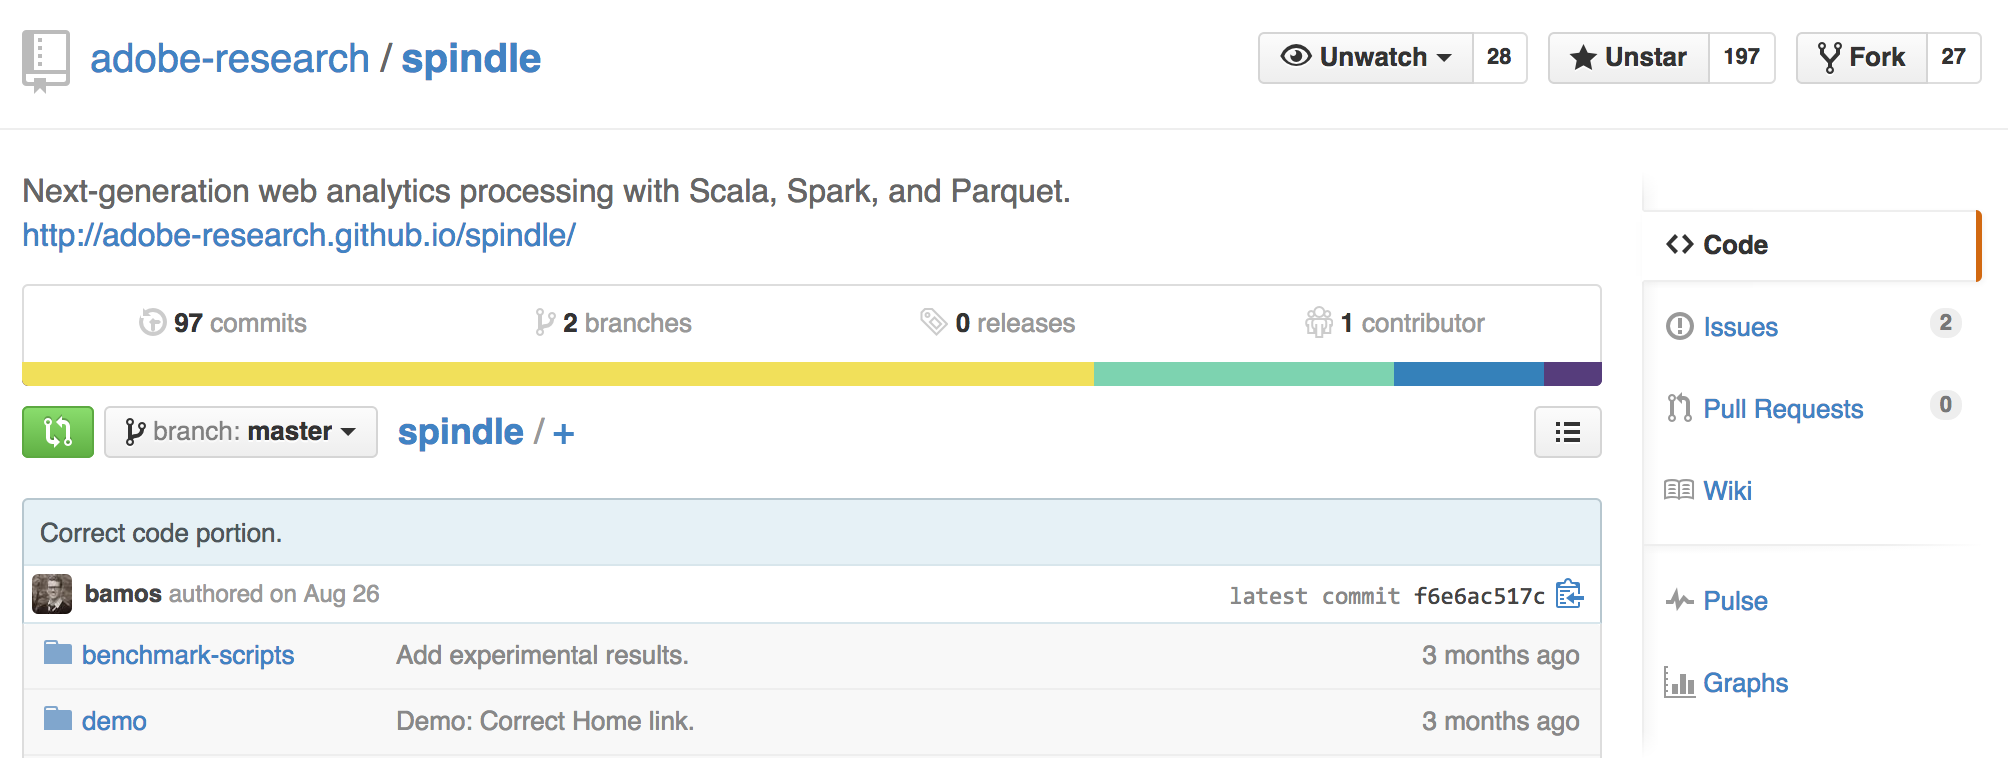
\includegraphics[width=0.9\textwidth]{spindle-github.png}
  \end{center}
}

\end{document}
